\section{Zbiory danych i metodyka}
\label{sec:metodyka}

Rozdział opisuje zbiory wzorców użyte w eksperymentach oraz wspólne dla wszystkich eksperymentów definicje: sposoby uszkadzania wejścia, klasy stanu końcowego i miary skuteczności. Na końcu zestawiono wszystkie przeprowadzone eksperymenty.

\subsection{Zbiory wzorców}
\label{sec:zbiory}

Do zadania dostarczono osiem zbiorów bitmap, pokazanych na Rysunku~\ref{fig:zbiory}. Zbiór \mbox{\texttt{small-7x7}} zawiera pięć prostych kształtów geometrycznych, \mbox{\texttt{letters-abc-8x12}} trzy małe litery a, b i c, \mbox{\texttt{animals-14x9}} sześć sylwetek zwierząt, a \mbox{\texttt{letters-14x20}} wszystkie 26 małych liter alfabetu łacińskiego. Zbiór \mbox{\texttt{OCRA-12x30-cut}} zawiera siedem wielkich liter kroju OCR-A przyciętych do \mbox{12x30} pikseli. Zbiór \mbox{\texttt{large-25x25}} to sześć większych obrazków (słońce, dom, szachownica, strzałka, pionowe pasy i napis z liter), a \mbox{\texttt{large-25x25.plus}} to te same obrazki i dziewięć kolejnych. Zbiór \mbox{\texttt{large-25x50}} zawiera obrazki z \mbox{\texttt{large-25x25}} w górnej połowie bitmapy, a dolna połowa jest w całości czarna. W nazwach zbiorów wymiary podano jako szerokość x wysokość, a piksel czarny odpowiada stanowi $+1$.

\begin{figure}[H]
    \centering
    \begin{subfigure}[b]{0.3\textwidth}
        \centering
        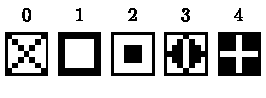
\includegraphics[width=\linewidth]{stability/figures/patterns-small-7x7.pdf}
        \caption{\texttt{small-7x7}}
    \end{subfigure}\hfill
    \begin{subfigure}[b]{0.22\textwidth}
        \centering
        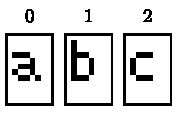
\includegraphics[width=0.909\linewidth]{stability/figures/patterns-letters-abc-8x12.pdf}
        \caption{\texttt{letters-abc-8x12}}
    \end{subfigure}\hfill
    \begin{subfigure}[b]{0.46\textwidth}
        \centering
        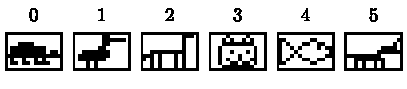
\includegraphics[width=\linewidth]{stability/figures/patterns-animals-14x9.pdf}
        \caption{\texttt{animals-14x9}}
    \end{subfigure}

    \medskip
    \begin{subfigure}[b]{0.45\textwidth}
        \centering
        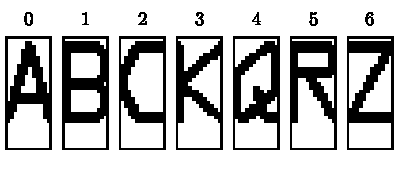
\includegraphics[width=\linewidth]{stability/figures/patterns-OCRA-12x30-cut.pdf}
        \caption{\texttt{OCRA-12x30-cut}}
    \end{subfigure}\hfill
    \begin{subfigure}[b]{0.53\textwidth}
        \centering
        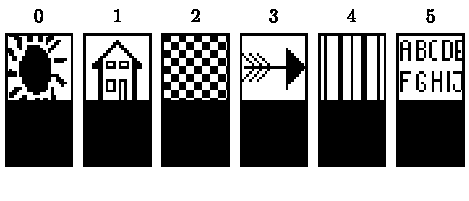
\includegraphics[width=\linewidth]{stability/figures/patterns-large-25x50.pdf}
        \caption{\texttt{large-25x50}}
    \end{subfigure}

    \medskip
    \begin{subfigure}[b]{\textwidth}
        \centering
        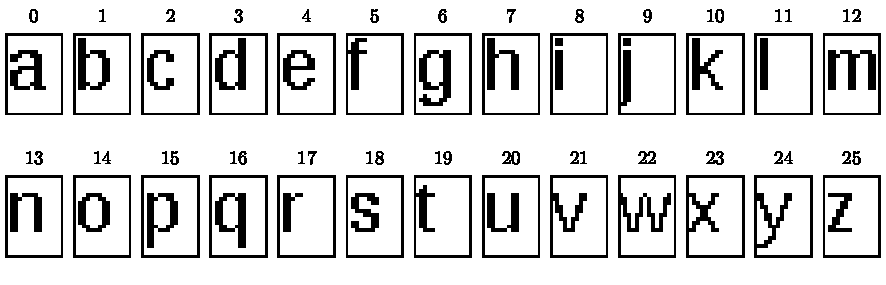
\includegraphics[width=\linewidth]{stability/figures/patterns-letters-14x20.pdf}
        \caption{\texttt{letters-14x20}}
    \end{subfigure}

    \medskip
    \begin{subfigure}[b]{\textwidth}
        \centering
        \includegraphics[width=\linewidth]{{stability/figures/patterns-large-25x25.plus}.pdf}
        \caption{\texttt{large-25x25.plus}, której pierwsze sześć wzorców tworzy zbiór \texttt{large-25x25}}
    \end{subfigure}
    \caption{Wzorce dostarczonych zbiorów. Nad każdą bitmapą podano numer wzorca w zbiorze.}
    \label{fig:zbiory}
\end{figure}

\noindent Liczbowe własności zbiorów zebrano w Tabeli~\ref{tab:zbiory}. Oprócz liczby wzorców $p$ i liczby neuronów $N$ podano obciążenie $p/N$, udział pikseli czarnych we wzorcach oraz średnią i największą wartość bezwzględną nakładania~\eqref{eq:nakladanie} między parami różnych wzorców. Nakładanie decyduje o wielkości składnika zakłócającego~\eqref{eq:przesluch}, więc jest głównym parametrem opisującym trudność zbioru dla reguły Hebba.

\begin{table}[H]
    \centering
    \caption{Własności zbiorów wzorców. Udział $+1$ to najmniejszy i największy udział pikseli czarnych we wzorcach zbioru, $\lvert m \rvert$ to wartość bezwzględna nakładania pary różnych wzorców.}
    \label{tab:zbiory}
    \small
    \begin{tabular}{l r r r r c r r}
        \toprule
        Zbiór & Wymiary & $p$ & $N$ & $p/N$ & Udział $+1$ & Śr. $\lvert m \rvert$ & Maks. $\lvert m \rvert$ \\
        \midrule
        \texttt{small-7x7} & \mbox{7x7} & 5 & 49 & \num{0.1020} & \numrange{0.184}{0.735} & \num{0.286} & \num{0.510} \\
        \texttt{letters-abc-8x12} & \mbox{8x12} & 3 & 96 & \num{0.0312} & \numrange{0.094}{0.146} & \num{0.806} & \num{0.833} \\
        \texttt{animals-14x9} & \mbox{14x9} & 6 & 126 & \num{0.0476} & \numrange{0.270}{0.397} & \num{0.212} & \num{0.381} \\
        \texttt{letters-14x20} & \mbox{14x20} & 26 & 280 & \num{0.0929} & \numrange{0.082}{0.229} & \num{0.728} & \num{0.986} \\
        \texttt{OCRA-12x30-cut} & \mbox{12x30} & 7 & 360 & \num{0.0194} & \numrange{0.283}{0.436} & \num{0.272} & \num{0.478} \\
        \texttt{large-25x25} & \mbox{25x25} & 6 & 625 & \num{0.0096} & \numrange{0.178}{0.501} & \num{0.142} & \num{0.469} \\
        \texttt{large-25x25.plus} & \mbox{25x25} & 15 & 625 & \num{0.0240} & \numrange{0.150}{0.501} & \num{0.171} & \num{0.498} \\
        \texttt{large-25x50} & \mbox{25x50} & 6 & 1250 & \num{0.0048} & \numrange{0.589}{0.750} & \num{0.567} & \num{0.734} \\
        \midrule
        \texttt{groups-25x25-d02} & \mbox{25x25} & 15 & 625 & \num{0.0240} & \numrange{0.285}{0.512} & \num{0.298} & \num{0.930} \\
        \texttt{groups-25x25-d05} & \mbox{25x25} & 15 & 625 & \num{0.0240} & \numrange{0.275}{0.518} & \num{0.263} & \num{0.834} \\
        \texttt{groups-25x25-d10} & \mbox{25x25} & 15 & 625 & \num{0.0240} & \numrange{0.310}{0.528} & \num{0.211} & \num{0.674} \\
        \texttt{groups-25x25-d20} & \mbox{25x25} & 15 & 625 & \num{0.0240} & \numrange{0.352}{0.518} & \num{0.126} & \num{0.405} \\
        \midrule
        \texttt{cats-300x200-median} & \mbox{300x200} & 12 & \num{60000} & \num{0.0002} & \numrange{0.486}{0.500} & \num{0.138} & \num{0.404} \\
        \texttt{cats-300x200-dither} & \mbox{300x200} & 12 & \num{60000} & \num{0.0002} & \numrange{0.356}{0.817} & \num{0.070} & \num{0.292} \\
        \bottomrule
    \end{tabular}
\end{table}

\noindent Wszystkie dostarczone zbiory mają obciążenie znacznie mniejsze niż granica $\num{0.138} N$ dla wzorców losowych, ale ich wzorce nie są losowe. Litery zajmują mały fragment bitmapy (od \qtyrange{8}{23}{\percent} pikseli czarnych w \mbox{\texttt{letters-14x20}}), więc dwie różne litery zgadzają się w większości pikseli wspólnego białego tła. Stąd średnie nakładanie $\num{0.806}$ w \mbox{\texttt{letters-abc-8x12}} i $\num{0.728}$ w \mbox{\texttt{letters-14x20}}, gdzie najbardziej podobna para liter ma $\lvert m \rvert = \num{0.986}$. Zbiory \mbox{\texttt{large-25x25}} i \mbox{\texttt{large-25x50}} zawierają te same obrazki, a mimo to średnie nakładanie w drugim jest około cztery razy większe, bo wspólna czarna połowa bitmapy jest identyczna we wszystkich wzorcach.

\subsection{Zbiory grupowe i zdjęcia}
\label{sec:zbiory-dodatkowe}

Do porównania zbioru z grupami podobnych wzorców ze zbiorem zróżnicowanym przygotowano cztery zbiory grupowe. Każdy powstał z trzech prototypów, obrazków 0, 2 i 4 ze zbioru \mbox{\texttt{large-25x25}}. Dla każdego prototypu utworzono pięć wariantów, w których odwrócono $\operatorname{round}(dN)$ losowo wybranych pikseli. Nakładanie wariantu z prototypem wynosi więc $1 - 2 \operatorname{round}(dN)/N$, czyli w przybliżeniu $1 - 2d$. Udział odwróconych pikseli wynosi $d = \num{0.02}$, $\num{0.05}$, $\num{0.1}$ albo $\num{0.2}$, a zbiory nazwano od tej wartości. Każdy zbiór grupowy ma tyle samo wzorców i neuronów co zróżnicowany zbiór \mbox{\texttt{large-25x25.plus}}, a różni się od niego tylko podobieństwem wzorców (Tabela~\ref{tab:zbiory}). Zbiór dla $d = \num{0.05}$ pokazano na Rysunku~\ref{fig:grupy}.

\begin{figure}[H]
    \centering
    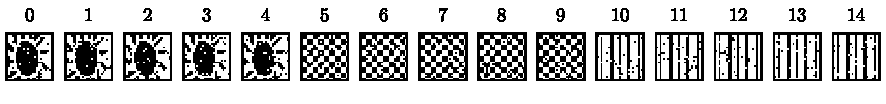
\includegraphics[width=\textwidth]{groups/figures/patterns-d05.pdf}
    \caption{Zbiór \texttt{groups-25x25-d05}: wzorce 0-4, 5-9 i 10-14 to warianty obrazków 0, 2 i 4 ze zbioru \texttt{large-25x25} z \qty{5}{\percent} odwróconych pikseli.}
    \label{fig:grupy}
\end{figure}

\noindent Eksperyment na dużych bitmapach przeprowadzono na dwunastu zdjęciach kotów z serwisu Wikimedia Commons, wymienionych w dodatku~\ref{app:zrodla-zdjec}. Każde zdjęcie przycięto do proporcji 3:2, przeskalowano do \mbox{300x200} pikseli ($N = \num{60000}$) i zamieniono na odcienie szarości. Zbiór \mbox{\texttt{cats-300x200-median}} powstał przez progowanie na medianie jasności zdjęcia, więc każda bitmapa ma prawie dokładnie połowę pikseli czarnych. Zbiór \mbox{\texttt{cats-300x200-dither}} powstał przez rozpraszanie błędu metodą Floyda-Steinberga (ang. \textit{dithering}), które oddaje jasność gęstością czarnych pikseli. Jego wzorce mają mniejsze nakładania, ale różne udziały pikseli czarnych (Tabela~\ref{tab:zbiory}). W obu zbiorach piksel ciemny odpowiada stanowi $+1$.

\subsection{Wejścia i uszkodzenia}
\label{sec:uszkodzenia}

Eksperymenty z odtwarzaniem składają się z prób. W jednej próbie każdy wzorzec zbioru po kolei jest celem: zostaje uszkodzony i podany sieci jako stan początkowy. Badano trzy rodzaje wejścia:
\begin{itemize}
    \item odwrócenie pikseli: zmienia się znak $\operatorname{round}(fN)$ losowo wybranych pikseli, gdzie $f \in [0; \num{0.5}]$ to poziom uszkodzenia (przy $f = \num{0.5}$ wejście jest średnio nieskorelowane z celem),
    \item zasłonięcie: pas $\operatorname{round}(fH)$ kolejnych wierszy na całej szerokości bitmapy, w losowym miejscu, zostaje ustawiony na $-1$ (biały), gdzie $H$ to wysokość bitmapy,
    \item wejście losowe: każdy piksel jest równy $+1$ albo $-1$ z prawdopodobieństwem $1/2$, niezależnie od wzorców.
\end{itemize}
Poziom zasłonięcia jest ułamkiem wierszy, a nie pikseli, więc nie jest porównywalny między zbiorami o różnych wymiarach. Pas zasłaniający zmienia tylko piksele czarne, więc liczba faktycznie zmienionych pikseli zależy od wzorca.

Eksperyment to siatka komórek, z których każda odpowiada jednej kombinacji zbioru, reguły uczenia, trybu dynamiki i poziomu uszkodzenia. W każdej komórce wykonuje się tę samą liczbę prób. Tryb synchroniczny bez uszkodzenia jest deterministyczny, więc w takiej komórce wykonuje się jedną próbę. Wejścia losuje się niezależnie od reguły i trybu (rozdział~\ref{sec:powtarzalnosc}), więc komórki różniące się tylko regułą lub trybem są porównywane na tych samych wejściach.

\subsection{Stany końcowe i miary skuteczności}
\label{sec:metryki}

Stan końcowy każdej próby trafia do jednej z pięciu klas: wzorzec (punkt stały równy któremuś wzorcowi zbioru), negacja wzorca, stan pozorny (każdy inny punkt stały), cykl długości 2 oraz brak zbieżności (osiągnięty limit kroków). Klasy są rozstrzygane przez dokładną równość stanów. Skuteczność oceniano następującymi miarami:
\begin{itemize}
    \item stabilność wzorca: wzorzec jest punktem stałym, gdy dla każdego piksela pole wyrównane $\xi^\mu_i h_i$ (pole lokalne pomnożone przez stan piksela we wzorcu) jest nieujemne, a piksel z ujemnym polem wyrównanym nazywa się niestabilnym,
    \item odsetek odzyskań: udział prób zakończonych punktem stałym równym celowi (bez uszkodzenia jest to odsetek stabilnych wzorców),
    \item odsetek prób zakończonych najbliżej celu: udział prób, w których stan końcowy ma z celem nakładanie dodatnie i nie mniejsze niż wartość bezwzględna nakładania z każdym innym wzorcem (miara przydatna, gdy cel nie jest stabilny, ale sieć kończy w stanie do niego podobnym),
    \item poziomy krytyczne $f_{0,9}$ i $f_{0,5}$: największy poziom uszkodzenia $f$, przy którym odsetek odzyskań wynosi co najmniej $\num{0.9}$ (odpowiednio $\num{0.5}$) dla $f$ i wszystkich mniejszych poziomów siatki (gdy warunek nie zachodzi już bez uszkodzenia, poziom krytyczny nie istnieje).
\end{itemize}

Odsetki podawane są z 95-procentowym przedziałem ufności Wilsona, danym wzorem~\eqref{eq:wilson}. Dla $k$ sukcesów w $n$ próbach, $\hat p = k/n$ i $z = \num{1.96}$ przedział ma środek i połowę szerokości
\begin{equation}
    \frac{\hat p + \frac{z^2}{2n}}{1 + \frac{z^2}{n}}, \qquad \frac{z}{1 + \frac{z^2}{n}} \sqrt{\frac{\hat p (1 - \hat p)}{n} + \frac{z^2}{4n^2}}.
    \label{eq:wilson}
\end{equation}
W odróżnieniu od przybliżenia normalnego przedział ten nie wychodzi poza $[0; 1]$ i nie ma zerowej szerokości dla odsetków 0 i 1, które w eksperymentach występują często. Komórki deterministyczne mają odsetki dokładne, bez przedziału.

\subsection{Przegląd eksperymentów}
\label{sec:eksperymenty}

Przeprowadzone eksperymenty zestawiono w Tabeli~\ref{tab:eksperymenty}. Nazwy odpowiadają katalogom z konfiguracjami i wynikami. Jeśli nie zaznaczono inaczej, każdy eksperyment obejmuje regułę Hebba i regułę Oji (wariant podprzestrzeni) w obu trybach dynamiki.

\begin{table}[H]
    \centering
    \caption{Eksperymenty. Poziomy podano jako zakres i krok. Próby to liczba prób w komórce (w każdej próbie każdy wzorzec jest raz celem), a dla wejścia losowego liczba wejść w komórce.}
    \label{tab:eksperymenty}
    \small
    \begin{tabularx}{\textwidth}{>{\ttfamily}l >{\raggedright\arraybackslash}X >{\raggedright\arraybackslash}p{4.1cm} r}
        \toprule
        \normalfont Eksperyment & Zbiory i reguły & Wejście, poziomy & Próby \\
        \midrule
        stability & 8 dostarczonych & bez uszkodzeń & 20 \\
        stability-single-neuron & 8 dostarczonych, tylko Oja jednoneuronowa & bez uszkodzeń & 20 \\
        capacity & prefiksy \texttt{letters-14x20} i \texttt{large-25x25.plus}, wzorce losowe ($N = 280$ i 625), tylko stabilność & brak & 50 \\
        large-recovery & \texttt{large-25x25}, \texttt{large-25x25.plus}, \texttt{large-25x50} & odwrócenie, \numrange{0}{0.5} co \num{0.05} & 100 \\
        noise & 8 dostarczonych & odwrócenie, \numrange{0}{0.5} co \num{0.05} & 100 \\
        occlusion & 8 dostarczonych & zasłonięcie, \numrange{0}{0.75} co \num{0.15} & 100 \\
        load & prefiksy \texttt{large-25x25.plus} ($p = 3, 6, 9, 12, 15$) i \texttt{letters-14x20} ($p = 2, 5, 10, 15, 20, 26$) & odwrócenie, \numrange{0}{0.5} co \num{0.05} & 100 \\
        groups & 4 grupowe i \texttt{large-25x25.plus} & odwrócenie, \numrange{0}{0.5} co \num{0.05} & 100 \\
        random & 8 dostarczonych & losowe & \num{10000} \\
        random-load & prefiksy jak w \texttt{load} & losowe & \num{10000} \\
        stable-5x5 & konstruowane zbiory bitmap \mbox{5x5}, tylko stabilność & brak & -- \\
        cycle & cztery kształty \mbox{5x5}, Hebb, tryb synchroniczny & szachownica & 1 \\
        cats-noise & 2 zbiory kotów & odwrócenie, \numrange{0}{0.5} co \num{0.05} & 100 \\
        cats-occlusion & 2 zbiory kotów & zasłonięcie, \numrange{0}{0.8} co \num{0.1} & 100 \\
        benchmark & wzorce losowe ($p = 12$, $N$ od \num{1024} do \num{60000}) i koty, czas i pamięć & odwrócenie, \num{0.1} & 5 \\
        \bottomrule
    \end{tabularx}
\end{table}
